\section{\acs{etl}-Strecke} \label{sec:etlpipeline}

Für den Import der Information der \ac{icd10gm} in der \ac{db} wurde eine \ac{etl}-Strecke entwickelt. Dazu wurden \ac{bash}-Skripts unter Ubuntu 20.04 programmiert und durchgeführt. Die Entscheidung von \ac{bash} basiert sich darauf, dass \ac{bash} die Standard interaktive Shell und Skript Sprache von Linux-Betriebssystemen ist und ermöglicht auch die Automatisierung einer Reihenfolge von Kommandos des Betriebssystems \cite{bash}. Da die Interaktion mit den Befehlen des Betriebssystems via \ac{bash} effizienter und leichter ist, ist es möglich in einer sicheren Art die Zugangsdaten für die \ac{db} zu nutzen, ohne diese Information in Klartext in den Skripten oder in anderen Dateien sichtbar zu platzieren.

Der Anfangspunkt für die Durchführung der \ac{etl} sind die ZIP-Dateien der Metadaten von 2007 bis 2021 aus der Download Seite vom \ac{bfarm} für die Klassifikationen. Diese Dateien wurden zuerst manuell heruntergeladen. Der Abruf und die Reihenfolge der Skripts für den Durchlauf jedes Schritts der \ac{etl} werden von einem zentralen \ac{bash}-Skript definiert. Die Abbildung~\ref{fig:etl} stellt das Flussdiagramm der \ac{etl}-Strecke dar.

\clearpage
\begin{figure}[ht]
	\centering
	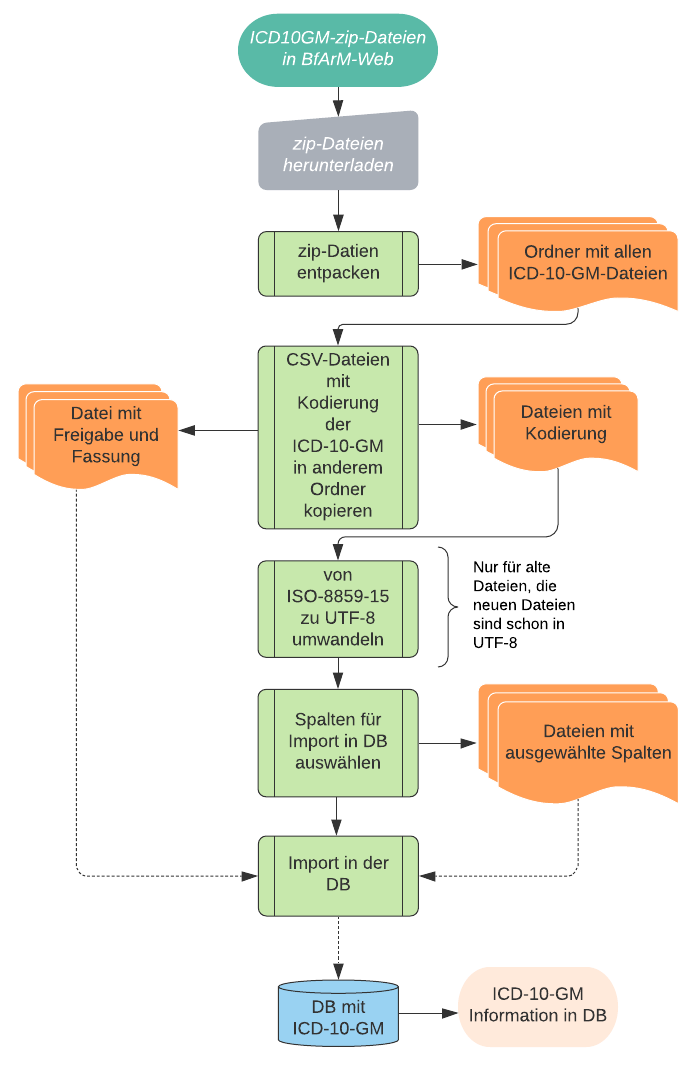
\includegraphics[height=14cm]{figures/etl}
	\caption[\acs{etl}-Strecke]{Flussdiagramm der \acs{etl}-Strecke für den Import der Informationen der \ac{icd10gm} aus den ZIP-Dateien in der \ac{db}.}
	\label{fig:etl}
\end{figure} 

\subsection{Extraktion} \label{subsec:extraction}

Zuerst werden die Ordner der ZIP-Dateien entpackt und ein neuer Ordner für die Speicherung der Kode-Dateien wird generiert. Diese Dateien werden ausgewählt und in den hergestellten Ordner kopiert. Die Information des Datums der Freigabe und Fassung wird aus der Liesmich-Datei extrahiert und in eine \ac{csv}-Datei importiert.

\subsection{Transformation} \label{subsec:transf}

Die Kode-Dateien von 2007 bis 2009 haben den Windows-Standardzeichensatz \acl{iso}, \acsu{iso}-8859-15 als Zeichenkodierung. Das verursacht Probleme bei dem Datenaustausch zwischen Plattformen, da die PostgreSQL Instanz in \acl{utf}, \acsu{utf}-8 konfiguriert ist. Aus diesem Grund wird das Format dieser Kode-Dateien von \ac{iso}-8859-15 in \ac{utf}-8 umgewandelt.

Im Laufe der Zeit sind neue Spalten in der \ac{csv}-Dateien der Klassifizierungen entstanden und andere Felder werden veraltet und entnommen \cite{readme13, readme17}. Deswegen werden die aktuell benutzten Spalten ausgewählt, leere Felder werden an den Positionen der Spalten, die vorher nicht vorhanden waren, eingefügt. Ein neues Feld mit der Version am Anfang jeder Zeile ist eingeführt, und der Datensatz mit den Änderungen in einer neuen generierten \ac{csv}-Datei gespeichert.

\subsection{Laden} \label{subsec:load}

Am Ende der Transformation wird die Information der zuletzt generierten \ac{csv}-Dateien mit Kodes in die Tabelle \glqq\textsf{kodes}\grqq{} der \ac{db} geschrieben. Der interne Datenfluss in der \ac{db} ist in der Sektion~\ref{sec:dbrun} beschrieben.